%・(4章と重複?要修正)

%・画面のレイアウトについて詳しく記述する

実験で使用するアプリケーションについて説明する.
画面は図\ref{GUI1}の様になっている.画面中央,やや上部に
zoomからOBS studioでキャプチャを行った,OmniEyeBall側の
THETA Vの映像を表示している.この際,本来はTHETA Vの映像は
縦横比$1:2$であるが,表示の際には上$frac{1}{5}$,下$frac{1}{5}$
を切り取って表示している.これは,2-1節で説明した,全天球カメラの
パノラマ映像の歪みに起因する.特に画面上部,下部の歪みが大きくなり,
接地面や天井のごく一部が拡大された,無意味な映像になってしまう.
そのため,視覚情報負荷を減らすために画像の一部を切り取った.

\begin{figure}[tbp]
  \centering
  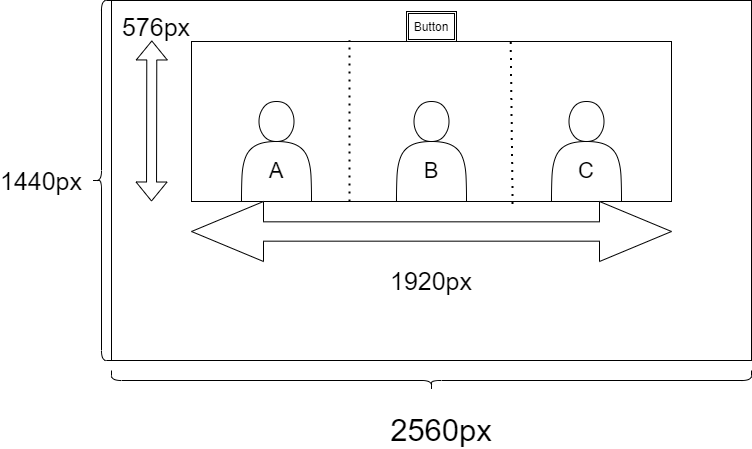
\includegraphics[scale=0.5]{fig/GUI1.png}\label{GUI1}
  \caption{GUIの模式図}
\end{figure}

実験では,OmniEyeBall使用者の人数,位置を固定し,図\ref{GUI1}
の点線で3等分している領域に映るようにした.(実際の画面では,点線に
相当するものは表示されない.)
各点線内部の領域をクリックし続けることが,領域内に映っている
参加者を見る,という行為に相当する.画面をクリックすると,
Tlinterの関数が呼び出され,クリック位置に応じた参加者が,
GUIに映る映像の中心に来る.(図\ref{GUI2})

\begin{figure}[tbp]
  \centering
  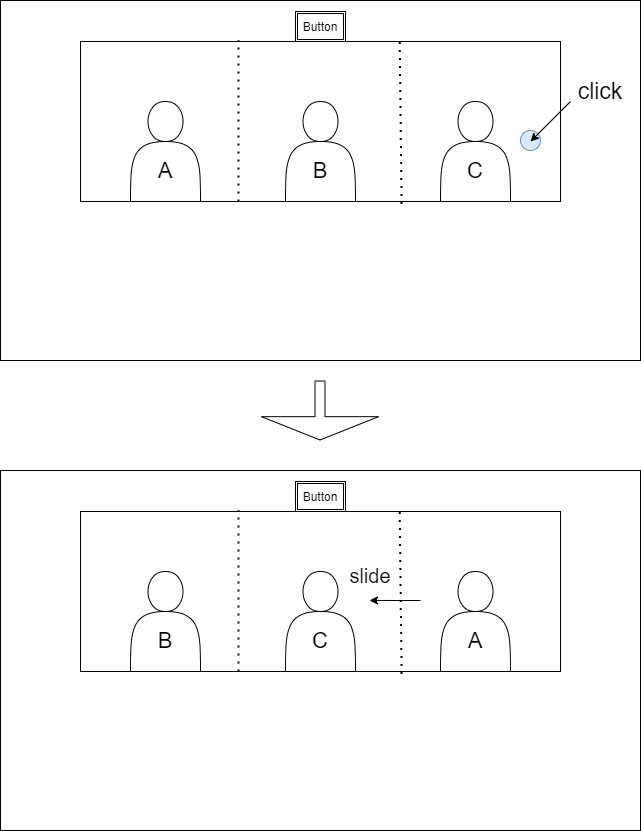
\includegraphics[scale=0.7]{fig/GUI2.png}
  \caption{中心へのスライド}\label{GUI2}
\end{figure}

この時,OmniEyeBall側では,表\ref{OEBGUI3}
の様に,クリックされている人物の方向へPC使用者の顔を表示させる.
図のA,Cの2人には
PC使用者と,クリックされている人物が会話中であるとみなし,
2つの小窓に2人の顔を表示した.顔画像は,映像の決まった位置から
OpenCVを用いてトリミング処理を行って作成した.

一方で,クリックを解除しているときは,PC使用者は
特定の個人を見ていないと判断し,3人全員に対して
PC使用者の顔の小窓を表示した.

\begin{figure}[tbp]
  \centering
  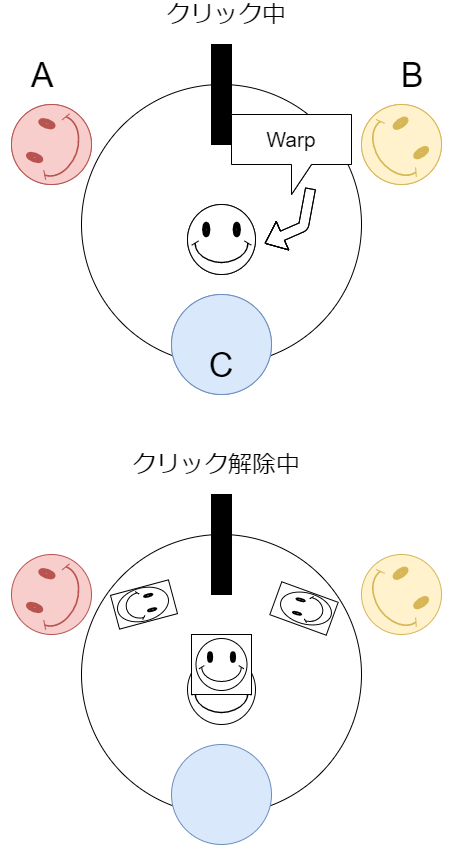
\includegraphics[scale=0.7]{fig/GUI3.png}
  \caption{OmniEyeBall上の表示変化}
\end{figure}

\begin{figure}[tbp]
  \centering
  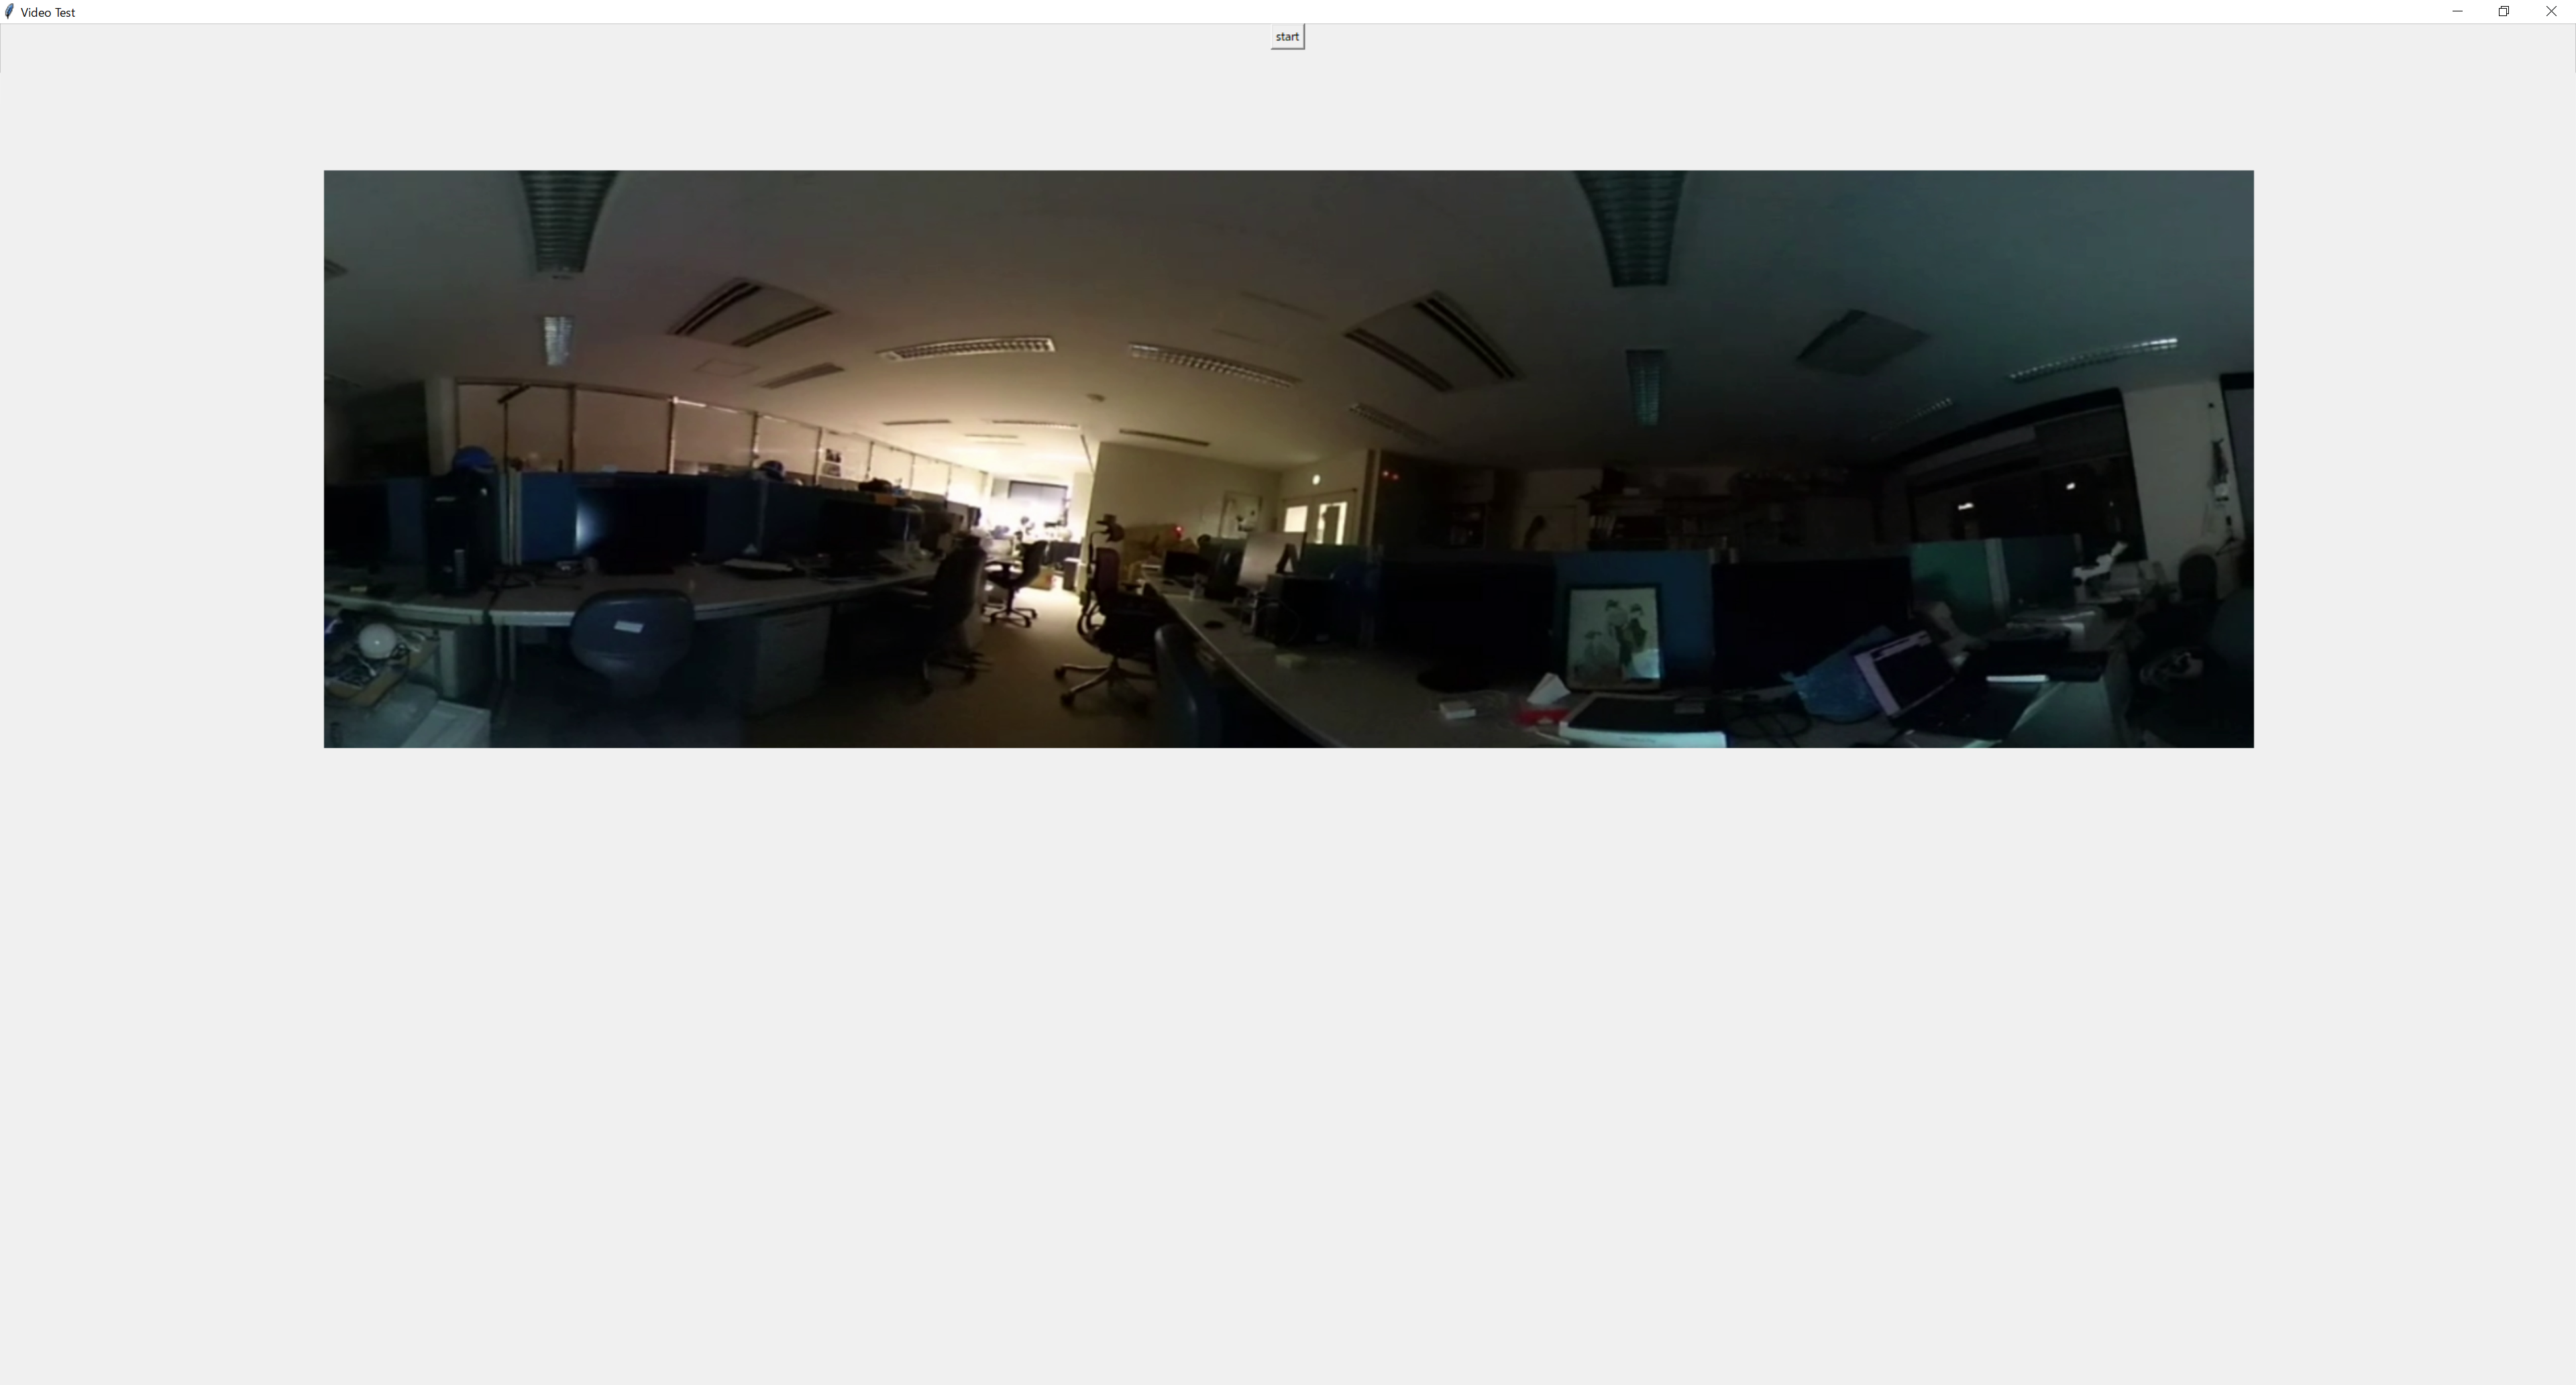
\includegraphics[scale=0.1]{fig/GUI.png}
  \caption{PC使用者に利用されるGUI画面}
\end{figure}

小窓の表示は,小窓の中心がOmniEyeBallの
北緯54度の緯線に重なる位置に表示した.

